\chapter{層の超局所台}
\section*{要約}
多様体\(X\)において，
\(\Dompb(X)\)の任意の対象\(F\)に対し，
\(T^{\ast}X\)の錐状閉部分集合を自然に対応させることができる．
この集合を\(F\)の超局所台といい，\(\muS(F)\)で表す．
大雑把に言って，
\(\muS(F)\)は\(X\)において\(F\)の「伝播しない」余方向を
記述するものであり，
後の章では，\(\muS(F)\)が\(T^{\ast}X\)の
包合的部分集合であることが示される．

この概念はまた，
層の理論における種々の関手が交換するための条件を与える．
例えば，\(f^{!}F\)が\(\omega_{Y/X}\tens[]f^{-1}F\)と
同型となるのはいつか？
あるいは\(f^{-1}\RHOM(F_1,F_2)\)が\(\RHOM(f^{-1}F,f^{-1}F)\)と
同型になるのはいつか？

ここではまず初めに\(\muS(F)\)の3つの定義が互いに同値であることを示し，
超局所台を用いて，\(X\)の開集合\(\varOmega_0\subset\varOmega_1\)に対し，
\(\RG(\varOmega_1;F)\)から
\(\RG(\varOmega_0;F)\)への制限射が同型になるための規準を与える．
第III章で閉凸固有錐\(\gamma\)から定まる\(\gamma\)位相を導入したが，
超局所台を調べる上ではこれが自然な道具である．
実際，\(X\)がアフィン空間で\(
    \phi_{\gamma}\colon X\to X_{\gamma}
\)が\(X\)の位相を弱める写像であるとき，\(
    \phi_{\gamma}^{-1}\Rder{{\phi_{\gamma}}_{\ast}}
\)は次の意味で切り落とし関手の役割を担う．\(
    \muS(\phi_{\gamma}^{-1}\Rder{{\phi_{\gamma}}_{\ast}}F)
\)が\(X\times\Int\gamma^{\circ a}\)に含まれ，射\(
    \phi_{\gamma}^{-1}\Rder{{\phi_{\gamma}}_{\ast}}F\to F
\)が「\(X\times\Int\gamma^{\circ a}\)における同型」となる．
本章では，この超局所的な同型を定義し，次章でその理論を展開する．

超局所台の例をいくつか見たのち，
テンソル積と\(\HOM\)，順像逆像，フーリエ佐藤変換といった，
層の演算に関する超局所台の振る舞いを調べる．

この章では，射はいつも固有であるか，
超局所台に関して「非特性的」であると仮定する．
第VI章ではこの制限は取り除く．
この章と次章で示す結果は，
解析的係数偏微分方程式論における古典的な結果の多くと非常に似通っている．
第XI章では，いくつかの古典的な結果を，超局所台の理論から導出する方法を述べる．

ここでは\cite{KS85}の理論展開にかなり忠実に従うが，
実際には，証明を単純化したところもいくつかある．

規約\ref{cnv40}を引き続き用いる．

\section{同値条件}
\begin{leftbar}
\begin{PRP}\label{prp511}
    \begin{enumerate}[(1)]
        \item \(\)\label{5111}
        \item \(\)\label{5112}
        \item \(\)\label{5113}
    \end{enumerate}
\end{PRP}
\end{leftbar}
\section{伝播}
\section{例：局所閉集合から定まる超局所台}

\begin{EG}
    \begin{figure}[htp]
        \centering
        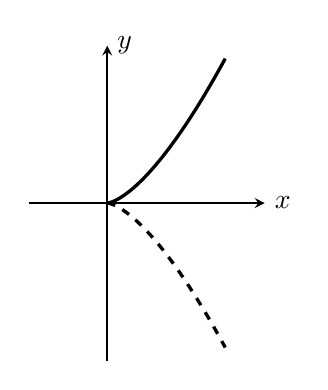
\begin{tikzpicture}
            \draw[->,>=stealth,semithick] (-1,0)--(2,0)node[right]{$x$}; %x軸
            \draw[->,>=stealth,semithick] (0,-2)--(0,2)node[right]{$y$}; %y軸
            %\draw (0,0)node[above  left]{O}; %原点
            %\fill[gray!20!white] plot[domain=0:3](\x,{sqrt(\x^3)});
            \draw[very thick,samples=100,domain=0:1.5] plot({\x},{sqrt(\x^3)}); 
            \draw[very thick,dashed,samples=100,domain=0:1.5] plot({\x},{-sqrt(\x^3)}); 
            %\draw (2*pi,0)node[below]{$2\pi$}; %点(2\pi,0)
            %\draw[dashed] (0,-1)node[left]{\(-1\)}--(1,-1)--(1,0)node[above]{$1$}; %点(1,-1)
            %\draw (2,0)node[above]{$2$}; %点(2,0)
        \end{tikzpicture}
        \caption{\(Z\)のグラフ}
    \end{figure}        
\end{EG}

\section{超局所台の関手的性質}

この節では，固有順像や非特性的の場合の逆像といった諸々の演算の下での
超局所台の振る舞いを調べる．
ここで得られる結果のいくつかは以降の章で一般化される．

\(X\)と\(Y\)を多様体とする．
これまで通り，\(X\times Y\)上で定義される
第1射影と第2射影を\(q_1\)と\(q_2\)で，
\(\cotb[X]\times \cotb[Y]\)上で定義される
第1射影と第2射影を\(p_1\)と\(p_2\)で表す．
\(f\)が\(Y\)から\(X\)への写像ならば，
第\ref{chap4}章のように，\(\mpb[f]\)と\(f_\pi\)で
以下の写像を表す．
\[
    \cotb[Y]
    \underset{\mpb[f]}{\longleftarrow}
    Y\pb[X]\cotb[X]
    \underset{f_{\pi}}{\longrightarrow}
    \cotb[X].
\]





\subsection*{テンソル積}


\begin{leftbar}
\begin{PRP}
    \(F\in\Dompb(X)\), \(G\in\Dompb(Y)\)ならば
    \[
        \muS\left(F\lletens[] G\right)
        \subset 
        \muS(F)\times\muS(G).
    \]
\end{PRP}        
\end{leftbar}

\begin{proof}
    \(X\)と\(Y\)はベクトル空間であると仮定してよい．
    \(
        (x_{\circ},y_{\circ};\xi_{\circ},\eta_{\circ})
        \in \cotb[(X\times Y)]
    \)とし，\((x_\circ;\xi_\circ)\notin\muS(F)\)であると仮定する．
    このとき，
    命題\ref{prp511}
    \eqref{5111}\(\Leftrightarrow\)\eqref{5113}
    より，
    \(x_{\circ}\)の開近傍\(U\)と
    実数\(\varepsilon>0\)と\(0\)を含む閉凸錐\(\gamma\)で，
    \begin{align*}
        H&=\{x;\langle x-x_\circ,\xi_{\circ}\rangle\geqq-\varepsilon\}, \\
        L&=\{x;\langle x-x_\circ,\xi_{\circ}\rangle=-\varepsilon\}    
    \end{align*}
    とおくとき，次をみたすものが存在する．
    \begin{itemize}
        \item \(\gamma-\{0\}\subset\left\{v;\langle v,\xi_{\circ}\rangle<0\right\}\)
        \item \(H\cap(U+\gamma)\subset X\)
        \item \(\RG(H\cap(x+\gamma);F)\simar\RG(L\cap(x+\gamma);F)\) (\(x\in U\))
    \end{itemize}
    この\(\gamma\)に対し\(
        \widetilde{\gamma}=\gamma\times\{0\}\subset X\times Y
    \)とおく．
    このとき\(z=(x,y)\in U\times Y\)に対して次が成り立つ．
    \begin{align}
        \RG\left(
            H\times Y\cap (z+\widetilde{\gamma});
            q_{1}^{-1}F\lltens[]q_{2}^{-1}G
        \right)
        &\cong
        \RG\left(H\cap (x+\gamma);F\lltens[]G_{y}\right)\tag{\(\ast\)}\label{eq:541-1}\\
        &\cong
        \RG(H\cap (x+\gamma);F)\lltens[]G_{y}.\tag{\(\ast\ast\)}\label{eq:541-2}
    \end{align}
    ただし，\(G_y\)は茎と定数層を同一視している．
    \(H\)を\(L\)にとりかえた\[
        \RG\left(
        L\times Y\cap (z+\widetilde{\gamma});
        q_{1}^{-1}F\lltens[]q_{2}^{-1}G
        \right)
        \cong
        \RG(L\cap (x+\gamma);F)\lltens[]G_{y}
    \]
    も同様に成り立つので．
    \[
        \RG(H\cap(x+\gamma);F)
        \simar
        \RG(L\cap(x+\gamma);F) 
    \]から\[
        \RG\left(
            H\times Y\cap (z+\widetilde{\gamma});
            q_{1}^{-1}F\lltens[]q_{2}^{-1}G
        \right)
        \cong
        \RG\left(
            L\times Y\cap (z+\widetilde{\gamma});
            q_{1}^{-1}F\lltens[]q_{2}^{-1}G
        \right)
    \]が成り立つ．
    したがって
    \(
        (x_{\circ},y_{\circ};\xi_{\circ},\eta_{\circ})
        \notin
        \muS\left(F\lletens[] G\right)
    \)となる．
\end{proof}
\begin{CMT}
    \(V=H\cap (x+\gamma)\)と略記する．

    1つ目の同型\eqref{eq:541-1}を示すには次の可換図式を考える．
    \[\vcenter{\xymatrix@C=26pt@R=26pt{
        V
        \ar@{^{(}->}[d]_-{i_{1}}
        \ar@/^1pc/[rr]^-{a_{V}}
        &
        V\times\{y\}
        \ar[l]^-{\widetilde{q}_{1}}
        \ar[r]_-{\widetilde{q}_{2}}
        \ar@{^{(}->}[d]^-{i}
        &
        \{y\}%\cong\{\pt\}
        \ar@{^{(}->}[d]^-{i_{2}}
        \\
        X
        &
        X\times Y
        \ar[l]^-{q_{1}}
        \ar[r]_-{q_{2}}
        &
        Y
    }}\]
    このとき\(\widetilde{q}_{1}\)が位相空間の同型であることと\[
        (H\times Y)\cap (z+\widetilde{\gamma})
        \cong
        H\cap (x+\gamma)\times\{y\}
    \]であることに注意しつつ，
    \begin{align*}
        \RG\left(
            H\times Y\cap (z+\widetilde{\gamma});
            q_{1}^{-1}F\lltens[]q_{2}^{-1}G
        \right)
        &=
        \RG\left(
            V\times\{y\};
            i^{-1}\left(q_{1}^{-1}F\lltens[]q_{2}^{-1}G\right)
        \right)\\
        &\cong
        \RG\left(
            V\times\{y\};
            i^{-1}q_{1}^{-1}F\lltens[]i^{-1}q_{2}^{-1}G
        \right)\\
        &\cong
        \RG\left(
            V\times\{y\};
            i^{-1}q_{1}^{-1}F\lltens[]i^{-1}q_{2}^{-1}G
        \right)\\
        &\cong
        \RG\left(
            V\times\{y\};
            \widetilde{q}_{1}^{-1}i_{1}^{-1}F\lltens[]\widetilde{q}_{2}^{-1}i_{2}^{-1}G
        \right)\\
        &\cong
        \RG\left(
            V\times\{y\};
            \widetilde{q}_{1}^{-1}i_{1}^{-1}F
            \lltens[]
            \widetilde{q}_{2}^{-1}G_{y}
        \right)\\
        &\cong
        \RG\left(
            V\times\{y\};
            \widetilde{q}_{1}^{-1}i_{1}^{-1}F
            \lltens[]
            \widetilde{q}_{1}^{-1}a_{V}^{-1}G_{y}
        \right)\\
        &\cong
        \RG\left(
            V\times\{y\};
            {\widetilde{q}_{1}}^{-1}\left(i_{1}^{-1}F
            \lltens[]
            a_{V}^{-1}G_{y}\right)
        \right)\\
        &\cong
        \RG\left(
            V;
            i_{1}^{-1}F\lltens[]a_{V}^{-1}G_{y}
        \right)
    \end{align*}
    である．
    2つ目の同型\eqref{eq:541-2}は\(V\)がコンパクトであることから射影公式を用いて
    \begin{align*}
        \RG\left(H\cap (x+\gamma);F\lltens[]a_{V}^{-1}G_{y}\right)
        &\cong
        \Rder{a_{V}}_{!}\left(F\lltens[]a_{V}^{-1}G_{y}\right)\\
        &\cong
        \Rder{a_{V}}_{!}F\lltens[]\Rder{a_{V}}_{!}a_{V}^{-1}G_{y}\\
        &\cong
        \RG(H\cap (x+\gamma);F)\lltens[]G_{y}
    \end{align*}
    が示せる．
\end{CMT}
\begin{CMT}
    \(
        (x_{\circ},y_{\circ};\xi_{\circ},\eta_{\circ})
        \notin
        \muS\left(F\lletens[] G\right)
    \)となる条件を詳しく確かめる．すなわち
    \(U\times Y\), \(\varepsilon>0\), 
    \(\widetilde{\gamma}\), \(H\times Y\), \(L\times Y\)は
    \begin{itemize}
        \item \(\widetilde{\gamma}-\{(0,0)\}
        \subset\left\{(v,w);
        \langle (v,w),(\xi_{\circ},\eta_{\circ})\rangle<0
        \right\}\)
        \item \((H\times Y)\cap(U\times Y+\tilde{\gamma})\subset X\times Y\)
    \end{itemize}
    をみたす．実際，1つ目は\[
        \widetilde{\gamma}-\{(0,0)\}
        =\left\{(v,w);
            v\in\gamma,\ w\in\{0\}, 
            v\ne0,w\ne0
        \right\}
        =(\gamma-\{0\})\times\varnothing=\varnothing
    \]なので成り立つ．
    \(U\times Y\)は，
    \(U\)が\(x_\circ\)の近傍なので，
    \((x_\circ,y_\circ)\)の近傍である．
    \(
        H\times Y\cap ((U\times Y)+\widetilde{\gamma})
        \subset X\times Y
    \)は\(X,\ Y\)をベクトル空間全体としていることから明らか．
\end{CMT}
\subsection*{Hom}
\subsection*{固有順像}
\subsection*{平滑射の逆像}
\begin{leftbar}
\begin{PRP}\label{prp545}
    \(f\colon Y\to X\)は平滑であるとする．
    \begin{enumerate}[(i)]
        \item \(F\in\Dompb(X)\)とする．このとき次が成り立つ．\[
            \muS(f^{-1}F)=\mpb[f](f_{\pi}^{-1}(\muS(F))).
        \]
        \item \(G\in\Dompb(Y)\)であるとき，
        次の条件\eqref{5452a}--\eqref{5452c}は互いに同値である．
        \begin{enumerate}[(a)]
            \item \(H^{j}(G)\)はすべて，
            \(f\)のファイバー上で局所定数層である，\label{5452a}
            \item \(Y\)上局所的に，\(G\cong f^{-1}F\)と
            なる\(F\in\Dompb(X)\)が存在する，\label{5452b}
            \item \(\muS(G)\subset \mpb[f](Y\times_X\cotb[X])\).\label{5452c}
        \end{enumerate}
    \end{enumerate}
\end{PRP}
\end{leftbar}

\begin{proof}
    (i) 
    逆の包含関係を示すには，命題5.1.1の条件(1)を用いる．
    \(\varphi\)が\(X\)上の\(C^1\)級関数で\(x\in X\)であるとき，
    任意の\(y\in f^{-1}(x)\)に対し次が成り立つことに注意すればよい．
    \[
        \left(\RG_{\{\varphi\geqq0\}}(F)\right)_{x}
        =
        \left(\RG_{\{\varphi\circ f\geqq0\}}(f^{-1}F)\right)_{y}.
    \]
\end{proof}

\begin{RMK}
    命題\ref{prp545}の状況のとき，
    \(V=\mpb[f](Y\times_{X}\cotb[X])\)とする．
    これは\(\cotb[Y]\)の滑らかな包合的部分多様体である．
    \(\muS(H^{j}(G))\subset \muS(G)\)は一般に成り立つとは
    限らない（注意5.1.4参照）が，
    命題\ref{prp545}から次が従う：\(
        \muS(G)\subset V
        \Leftrightarrow \text{任意の\(j\)に対し，}
        \muS(H^{j}(G))\subset V.
    \)
\end{RMK}

層理論における種々の演算の下での超局所台の振る舞いを表すために，
新しい記法を導入する．\(\cotb[X]\)の錐\(A\)と\(B\)に対して\(A+B\)を
次で定める．
\begin{equation}
    (A+B)\cap\pi^{-1}(x)\coloneqq
    \left\{
        a+b~;~ 
        a\in A\cap \pi^{-1}(x),~ 
        b\in B\cap \pi^{-1}(x)
    \right\}.
\end{equation}

\begin{leftbar}
\begin{LMM}
    \(A\)と\(B\)が\(\cotb[X]\)の閉錐で\(
        A\cap B^{a}\subset \cotz[X]
    \)をみたすとき，
    \(A+B\)も\(\cotb[X]\)の閉錐である．
\end{LMM}
\end{leftbar}

\clearpage
\section{錐状層の超局所台}
\newcommand{\eu}{\mathbf{e}}
\newcommand{\rrp}{\rr^{+}}

この節ではベクトル束上の層の超局所台について調べる．

\(\tau\colon E\to Z\)を多様体\(Z\)上の
実ベクトル束とする（III \S7参照）．
\(\rrp\)の\(E\)への作用を表す写像を\(
    \mu\colon \rrp\times E\to E
\)で表し，
\(\mu\)の無限小作用を表す\(E\)上のベクトル場
を\(\eu\)で表す．
すなわち\(E\)上の任意の関数\(\varphi\)に対し，\(
    (\eu(\varphi))(x)
    =
    \dfrac{\partial}{\partial{t}}\varphi(\mu(t,x))|_{t=1}
\)が成り立つ．
ベクトル場\(\eu\)は
\textbf{オイラーベクトル場} (the Euler vector field) と
呼ばれることが多い．
写像\(\mu\)から写像\(
    \mpb[\mu]\colon
    \rrp\times\cotb[E]\to\cotb[\rrp]\times\cotb[E]
\)が定まる\footnote{
    ここで，\(
        \mpb[\mu]\colon(\rrp\times E)\times_{E}\cotb[E]
        \to
        \cotb[\rrp]\times\cotb[E]
    \)の源\((\rrp\times E)\times_{E}\cotb[E]\)と\(
        \rrp\times\cotb[E]
    \)を同型\[
        \left(
            \left(t,\left(x;v\right)\right),
            \left(\left(x;v\right);\xi\right)
        \right)
        \leftrightarrow
        \left(
            t,
            \left(\left(x;v\right);\xi\right)
        \right)
    \]によって同一視している．
}．\(\mpb[\mu]\)の\(1\in\rrp\)への制限を考え，射影\(
    \cotb[\rrp]\times\cotb[E]
    \to
    \cotb[\rrp]\cong\rrp\times\rr\to\rr
\)と合成することにより，写像\begin{equation}
    \theta_{E}\colon\cotb[E]\to\rr
\end{equation}を得る．
この写像は\(\eu\)の主要表象に他ならない．

\((z,x)\)を（\(Z\)上局所的な）座標系で，
\((z)\)が\(Z\)の座標で\((x)\)が線形座標であるものとする．
\((z,x;\zeta,\xi)\)で対応する\(\cotb[E]\)の座標を表す．
このとき，
\begin{equation}
    \begin{dcases}
        \eu=\left\langle{x,\dfrac{\partial}{\partial{x}}}\right\rangle=\sum_{j}x_{j}\dfrac{\partial}{\partial{x_{j}}},\\
        \theta_{E}=\left\langle{x,\xi}\right\rangle,\\
        \alpha_{E}=\left\langle{\zeta,dz}\right\rangle+\left\langle{\xi,dx}\right\rangle
    \end{dcases}
\end{equation}
である．
ただし，\(\alpha_{E}\)は\(\cotb[E]\)の標準\(1\)形式である
（A\S2参照）．

\(\cotb[(E/Z)]\)で\(Z\)上の\(E\)の相対余接束を表していた．
これは\(E\)上のベクトル束の完全列
\begin{equation}
    0\to E\pb[Z]\cotb[Z]\to\cotb[E]\to\cotb[(E/Z)]\to0
\end{equation}
で定義される．
任意の\(z\in Z\)に対し，
\(\cotb[(E/Z)]\)の\(z\)上のファイバー\(\cotb[(E/Z)]_{z}\)は
\(E\)の\(z\)上のファイバー\(E_{z}\)の余接束\(\cotb[(E_{z})]\)と
同一視できる．
他方で，\(\cotb[(E_{z})]\)は\(E_{z}\times E^{\ast}_{z}\)と
同型である．
したがって，各\(z\)に対し，
\(\cotb[(E/Z)]_{z}\)から\(E^{\ast}_{z}\)への写像が定まる．
これから写像\begin{equation}
    \cotb[(E/Z)]\to E^{\ast}
\end{equation}がえられる．このとき\(Z\)上の射
\begin{equation}
    \psi_{E}\colon\cotb[E]\to E^{\ast}
\end{equation}
を\(\cotb[E]\to \cotb[(E/Z)]\to E^{\ast}\)の合成として定める．


\begin{leftbar}
\begin{PRP}\label{prp551}
    \begin{enumerate}[(i)]
        \item 写像\(\varPhi\colon \cotb[E]\to\cotb[E]\)で，
        \(
            \alpha_{E}-d\theta_{E}
            =\varPhi_{E}^{\ast}(\alpha_{E^{\ast}})
        \)であり\(
            \cotb[E]\underset{\varPhi_{E}}{\rightarrow}
            \cotb[E^{\ast}]\underset{\alpha}{\rightarrow}
            E^{\ast}
        \)の合成が\(\psi_{E}\)となるものがただひとつ存在する．
        \item \(\theta_{E^{\ast}}\circ\varPhi_{E}=-\theta_E\)である．
        \item \(\varPhi_{E^{\ast}}\circ \varPhi_{E}=-a^{\ast}\)である．ただし，\(a^{\ast}\)は\(E\)上の対蹠写像からひきおこされる\(\cotb[E]\)の自己同型である．
    \end{enumerate}
\end{PRP}
\end{leftbar}
    
\begin{proof}
    \begin{equation}
        \varPhi_{E}\colon (z,x;\zeta,\xi)\mapsto(z,\xi;\zeta,-x)
    \end{equation}
\end{proof}

\begin{RMK}\label{rmk552}
    \(\varPhi_{E}\)はシンプレクティック変換だが
    斉次シンプレクティック変換ではない．
\end{RMK}

\begin{equation}
    S_{E}=\theta_{E}^{-1}(0)
\end{equation}

\begin{equation}
    \begin{dcases}
        (z,x;\zeta,\xi)\mapsto (z,x;\lambda\zeta,\lambda\xi),& \lambda\in\rrp,\\
        (z,x;\zeta,\xi)\mapsto (z,\mu x;\zeta,\mu^{-1}\xi),& \mu\in\rrp.
    \end{dcases}
\end{equation}

\begin{leftbar}
\begin{PRP}\label{prp553}
    \begin{enumerate}[(i)]
        \item \(\Dbconic(E)\)
        \item \(F\in\Dbconic(E)\)のとき，\(\muS(F)\)は2重錐状
    \end{enumerate}
\end{PRP}
\end{leftbar}
    
\begin{equation}
    \vcenter{\xymatrix{
        \cotb[E]
        &
        E\pb[Z]\cotb[Z]
        \ar@{_{(}->}[l]-^{\mdiff[\tau]}
        &
        \cotb[Z]\\
        \ar@{_{(}->}[u]-^{\mdiff[\dot{\tau}]}
        \cotb[{\dot{E}}]
        &
        \ar@{_{(}->}[u]-^{\mdiff[\dot{\tau}]}
        \ar@{_{(}->}[l]-^{\mdiff[\dot{\tau}]}
        \dot{E}\pb[Z]\cotb[Z]
        &
        \ar@{_{(}->}[u]-^{\mdiff[\dot{\tau}]}
        \cotb[Z].
    }}
\end{equation}

\begin{equation}
    \cotb[Z]\hookrightarrow
    E\pb[Z]\cotb[Z]
    \underset{\mdiff[\tau]}{\hookrightarrow}
    \cotb[E].
\end{equation}



\begin{equation}
    \mpb[\tau]\mdiff[\tau]^{-1}(A)=\cotb[Z]\cap A.
\end{equation}

\begin{leftbar}
\begin{PRP}
    \(F\in\Dbconic(E)\)とする．このとき，次がなりたつ．
    \begin{enumerate}[(i)]
        \item \(\muS(\Rder{\tau_{\ast}}(F))\subset \cotb[Z]\cap\muS(F)\),
        \item \(\muS(\Rder{\tau_{!}}(F))\subset \cotb[Z]\cap\muS(F)\),
        \item \(\muS(\Rder{\dot{\tau}_{\ast}}(F))\subset \mpb[\dot{\tau}]\mdiff[\dot{\tau}]^{-1}(\muS(F))\),
        \item \(\muS(\Rder{\dot{\tau}_{!}}(F))\subset \mpb[\dot{\tau}]\mdiff[\dot{\tau}]^{-1}(\muS(F))\).
    \end{enumerate}
\end{PRP}
\end{leftbar}


\begin{leftbar}
\begin{THM}
    \(F\in\Dbconic(E)\)とする．
    \(\cotb[E]\)と\(\cotb[E^{\ast}]\)を\(\varPhi_{E}\)で
    同一視することにより，
    次がなりたつ．
    \[
        \muS(F)=\muS(F^{\wedge}).
    \]
\end{THM}
\end{leftbar}

\begin{proof}
    \begin{align}
        x_{\circ}\ne0,
        \quad
        \xi_{\circ}\ne0,\label{eq:5512}\\
        \RG_{Z}(F)=0.\label{eq:5513}    
    \end{align}
\end{proof}
